\documentclass[a4paper]{article}

%%%%%%%%%%%%%%%%
%%% PREAMBLE %%%
%%%%%%%%%%%%%%%%

%%% PACKAGES %%%
\usepackage{fontspec}                     % set fonts
	\setmainfont{Junicode}
\usepackage[a4paper,margin=3cm]{geometry} % page layout
\usepackage[svgnames]{xcolor}             % rainbowssss *_*
\usepackage{hyperref}                     % enhanced references (links)
	\hypersetup{%
		colorlinks=true,
		allcolors=NavyBlue}
\usepackage{fancyhdr}                     % headers & footers
\usepackage{titling}                      % macros \thetitle, \theauthor
\usepackage{graphicx}                     % enhanced graphics support
	\graphicspath{{img/}}
\usepackage[toc]{glossaries}              % glossaries (obv)
	\setglossarystyle{altlisthypergroup}
	\makeglossaries
	\newglossaryentry{turnstile}
{%
	name=turnstile,
	description={An ingress control device to help with the organizization
	of the passengers’ boarding. Basically a lockable revolving gate with
	three arms. When signalled, the gate unlocks and a single passenger may
	go through by turning one of the arms. After a single rotation, the gate
	locks again, waiting for the next signal.}
}

\newglossaryentry{authentication}
{%
	name=authentication,
	description={The process of verifying the \textit{identity} of the
	passengers.}
}

\newglossaryentry{authorization}
{%
	name=authorization,
	description={The process of veryfying whether an identified passenger
	has \textit{permission} to do something (eg board the bus).}
}

\newglossaryentry{alarm}
{%
	name=alarm,
	description={A device installed at every door that emits light and sound
	to draw attention to certain events. For instance, it signals the end of
	the boarding phase and also turns on in the event of an unauthorized
	boarding attempt.}
}

\newglossaryentry{RFIDScanner}
{%
	name={RFID scanner},
	description={An instrument capable of reading radio frequency
	identification tags. This can be used to effectively identify
	passengers.}
}

\newglossaryentry{boardingController}
{%
	name={boarding controller},
	description={A device responsible for the orchestration of the whole
	boarding phase (signalling doors to open or close, activating the alarm,
	etc).}
}

\usepackage{enumitem}                     % enhanced enumerations
\usepackage{tabularx}                     % enhanced tables
\usepackage{float}                        % 'H' figure placement
\usepackage{rotating}                     % sidewaysfigure
\usepackage[noabbrev]{cleveref}           % clever references
\usepackage{booktabs}                     % pretty tables
\usepackage{tikz}                         % drawings
	\usetikzlibrary{shapes}

%%% OTHER %%%
\setlength\headheight{22.3725pt}

%%% META %%%
\title{Assignment \#2 \\ Structural Modelling of Functional Units}
\author{Levendula}
\date{\today}

%%% ADDITIONAL PACKAGE CONFIG %%%
% fancyhdr
\pagestyle{fancy}
\fancyhf{}
\lhead{\theauthor}
\rhead{\thetitle}
\lfoot{\today}
\rfoot{\thepage}

%%%%%%%%%%%%%%%%%%%%%%%%%%%%%%%%%%%%%%%%%%%%%%%%%%%%%%%%%%%%%%%%%%%%%%%%%%%%%%%%

%%%%%%%%%%%%
%%% BODY %%%
%%%%%%%%%%%%

\begin{document}

\begin{titlepage}
	\begin{center}
		
\includegraphics[width=8cm]{logo.jpg}

		\vspace{.2cm}

		\textbf{Budapest University of Technology and Economics} \\
		Faculty of Electrical Engineering and Informatics \\
		Department of Measurement and Information Systems \\

		\vspace{2cm}

		{\huge IT System Design (\texttt{VIMIAC01})}

		\vspace{2cm}

		{\huge \bfseries \thetitle}

		\vspace{.5cm}

		{\Large \theauthor}

		\vspace{.5cm}

		{\Large \today}
	\end{center}

	\vfill{}

	{\large Team members:}

	\vspace{.25cm}

	\begin{tabular}{lll}
		Annamária Gálik &
			\texttt{WGMUO2} &
			ancsi666@gmail.com \\
		Borbála Szilágyi &
			\texttt{COVQ1M} &
			szilagyiborbala8@gmail.com \\
		Bertalan Z. Péter &
			\texttt{QO7CU6} &
			bertalan.peter+uni@bertalanp99.eu
	\end{tabular}

	\vspace{2cm}
\end{titlepage}


\tableofcontents
\listoffigures
\clearpage

% ------------------------------------------------------------------------------
\section{Our task}

Our job was to design crucial functional components including a couple of
subsystems for the IntelliBus system.

First, we had to complete the Block Definition Diagram of the \emph{Automated
Passenger Counting} functionality with traceability relationships between the
requirements and design artefacts. Documentation for this subtask can be found
at \cref{subsec:apc}.

Our next task was the bottom-up design of an \emph{Intelligent Intersection
Control} subsystem. We realized a specific junction—named J42— using the
conponents defined in the vendor catalog (which was given to us in the form of a
Block Definition Diagram). See our solution at \cref{subsec:j42}.

Finally, we created the top-down design of the \emph{Traffic and Route Planning}
functionality. For this task we used information and components provided by the
two previous tasks. See \cref{subsec:trp}.

% TODO uncomment ha csináltuk
%After designing
%the components we specified well-formedness constraints for the system model.



% ------------------------------------------------------------------------------
\section{Ambiguities and our ideas}

% TODO
\begin{enumerate}
	\item The layout of the T-intersection (J42)

		\textit{Each of the three roads has one incoming and one
			outgoing lane and there are three pedestrian
			crossings—one for each road.}
\end{enumerate}



% ------------------------------------------------------------------------------
\section{Solutions}

\subsection{Traceability links for the Automated Passenger Counting (APC)}%
\label{subsec:apc}

As per requirement \texttt{REQ1.1}, the buses must monitor the number of
passengers boarding and alighting. This is realized by the
\texttt{PassengerCounter} component which is to be installed into the doors of
every vehicle. There is an extra dependability requirement for this counting
functionality, which of course also must be safisfied by the
\texttt{PassengerCounter}.

\sloppy
The \texttt{PassengerCounter} is a special kind of \texttt{PassengerDetector}.
Another kind is the \texttt{PassengerRecognizer}, which is responsible not for
counting the passengers, but idefntifying them in order to keep track of who is
where. Requirement \texttt{REQ1.2} expects this functionality, which is
satisfied by this component. Similarly to \texttt{REQ1.1}, the dependability
requirement is also satisfied by the recognizer component. Also, all buses have
\texttt{PassengerRecognizer}s installed at every door.

Lastly, as requirement \texttt{REQ1.3} states, data collected by passenger
monitoring must be reported to a central system. This is done by the
\texttt{PassengerMonitoringModule}, which is responsible for keeping track of
passengers in general.

\begin{sidewaysfigure}
	\centering
	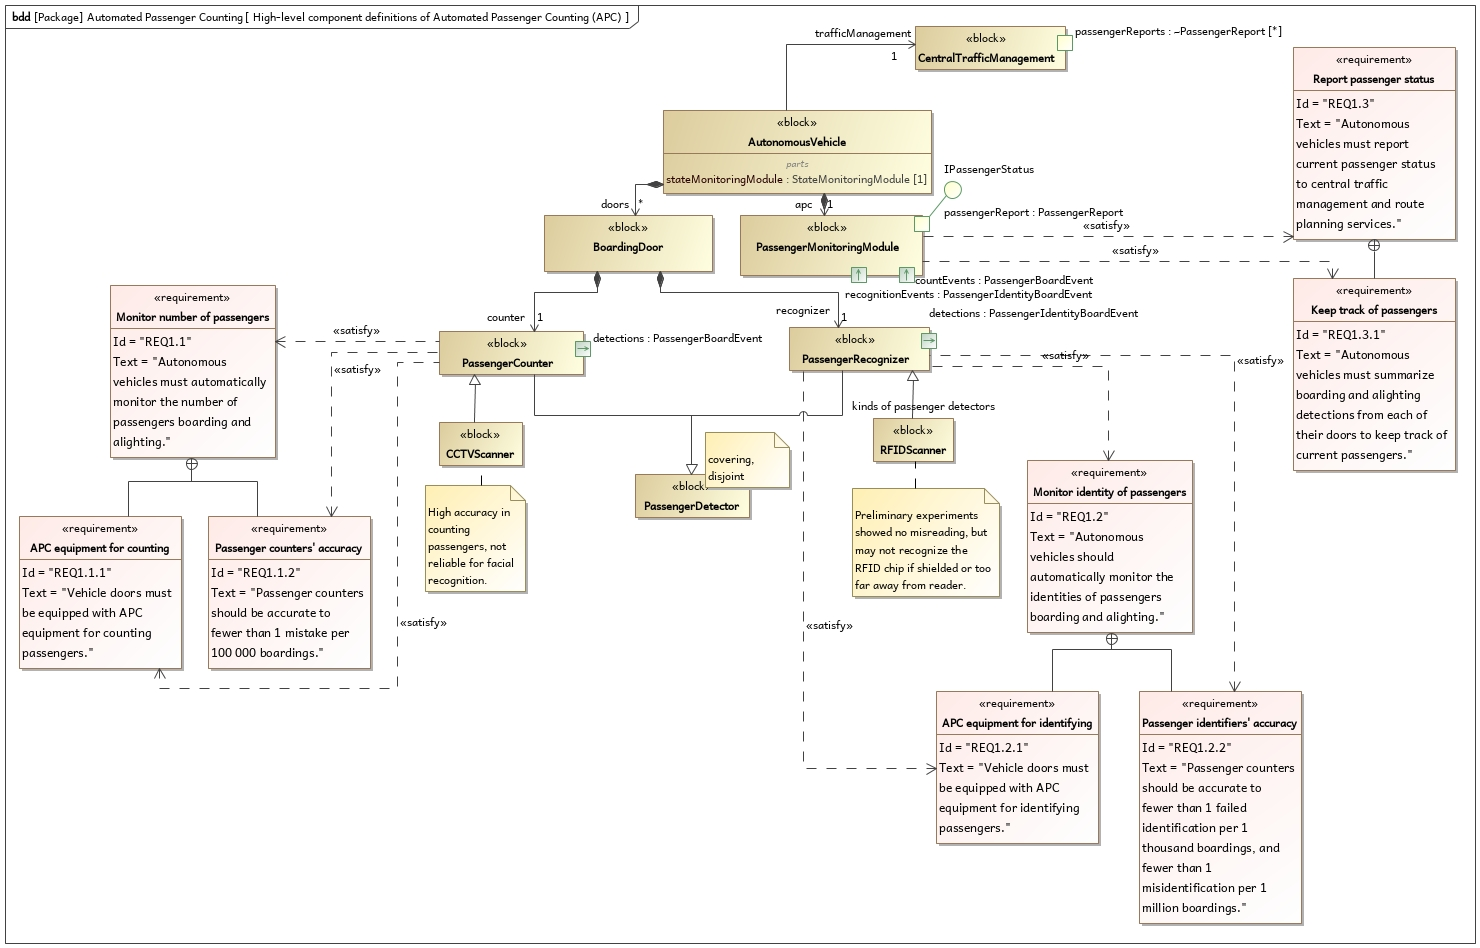
\includegraphics[width=\textwidth]{bdd-apc.jpg}
	\caption{High-level component definitions of the Automated Passenger
		Counting}%
	\label{fig:bdd-apc}
\end{sidewaysfigure}


% - - - - - - - - - - - - - - - - - - - - - - - - - - - - - - - - - - - - - - -
\subsection{Junction \#42 structure (IIC)}
\label{subsec:j42}

Junction 42 is a simple T-intersection, where a road coming from the west meets
a north to south road. We imagined the intersection layout as seen on
\cref{fig:j42}. Each of the three arms has a pedestrian crossing and a traffic
light (represented as a red triangle in the figure).

\begin{figure}[h]
	\centering
	\begin{tikzpicture}[%
		scale=.4,
		road/.style={very thick},%
		zebra/.style={thick},%
		lamp/.style={%
			scale=.5,
			draw,%
			regular polygon,%
			regular polygon sides=3,%
			fill=red}
		]

		% west lane
		\draw[road] (1,4)--(4,4);
		\draw[road] (1,6)--(4,6);
		% north–south lane
		\draw[road] (4,9)--(4,6);
		\draw[road] (4,4)--(4,1);
		\draw[road] (6,9)--(6,1);
		% west pedestrian crossing
		\draw[zebra] (2.5,4.4)--(3.5,4.4);
		\draw[zebra] (2.5,4.8)--(3.5,4.8);
		\draw[zebra] (2.5,5.2)--(3.5,5.2);
		\draw[zebra] (2.5,5.6)--(3.5,5.6);
		% north pedestrian crossing
		\draw[zebra] (4.4,7.5)--(4.4,6.5);
		\draw[zebra] (4.8,7.5)--(4.8,6.5);
		\draw[zebra] (5.2,7.5)--(5.2,6.5);
		\draw[zebra] (5.6,7.5)--(5.6,6.5);
		% south pedestrian crossing
		\draw[zebra] (4.4,3.5)--(4.4,2.5);
		\draw[zebra] (4.8,3.5)--(4.8,2.5);
		\draw[zebra] (5.2,3.5)--(5.2,2.5);
		\draw[zebra] (5.6,3.5)--(5.6,2.5);
		% traffic lights
		\node[lamp,rotate=-90] at (2,4.5) {};
		\node[lamp] at (4.4,8) {};
		\node[lamp,rotate=180] at (5.6,2) {};
	\end{tikzpicture}
	\caption{Our interpretation of J42's layout}%
	\label{fig:j42}
\end{figure}

We have created the Internal Block Diagram seen on \cref{fig:ibd-j42}. We
included the various control and information flows between the modules. The
traffic light at each pedestrian crossing is influenced by the pedestrian call
buttons. Each lane is also equipped with a vehicle detector.

\begin{sidewaysfigure}
	\centering
	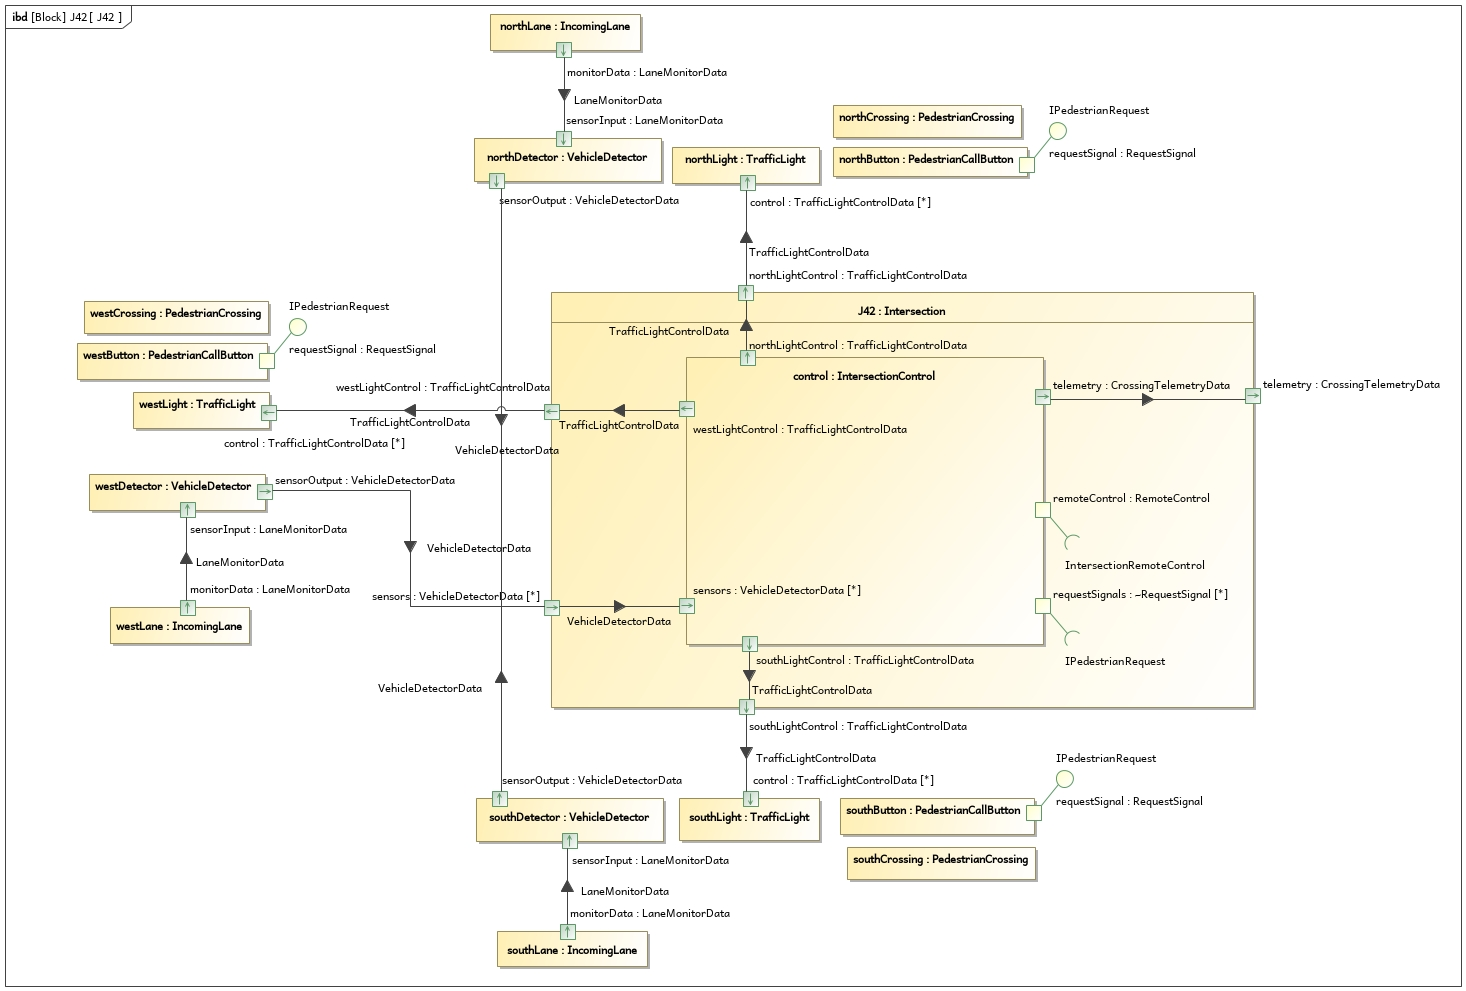
\includegraphics[width=\textwidth]{ibd-j42.jpg}
	\caption{Internal Block Diagram for the J42 junction}
	\label{fig:ibd-j42}
\end{sidewaysfigure}


% - - - - - - - - - - - - - - - - - - - - - - - - - - - - - - - - - - - - - - -
\subsection{Traffic and Route Planning}%
\label{subsec:trp}

As the most complicated task, we had to design the structural model of the
Traffic and Route Planning functionality.

Please see a Block Definition Diagram on \cref{fig:bdd-trp} which includes all
components used. The functionality is described on the following four Internal
Block Diagrams:

\begin{enumerate}
	\item \texttt{IntersectionControl}

		Explains the relations and communication between the central
		traffic management system and intersection control units. See
		\cref{fig:ibd-intersectioncontrol}.

	\item \texttt{Maintenance}

		Communication between the autonomous vehicles and maintenance
		manager components. See \cref{fig:ibd-maintenance}.

	\item \texttt{RoutePlanning}

		An functionality of crucial importance is the ability to devise
		routes based on various factors. The
		\texttt{ServiceRoutePlanner} is largely responsible for this.
		Find the diagram on \cref{fig:ibd-routeplanning}.

	\item \texttt{TrafficManagement}

		Explains the internal structure of the central traffic
		management component and how it communicates with sensors and
		vehicles. See \cref{fig:ibd-trafficmanagement}.
\end{enumerate}

\begin{sidewaysfigure}
	\centering
	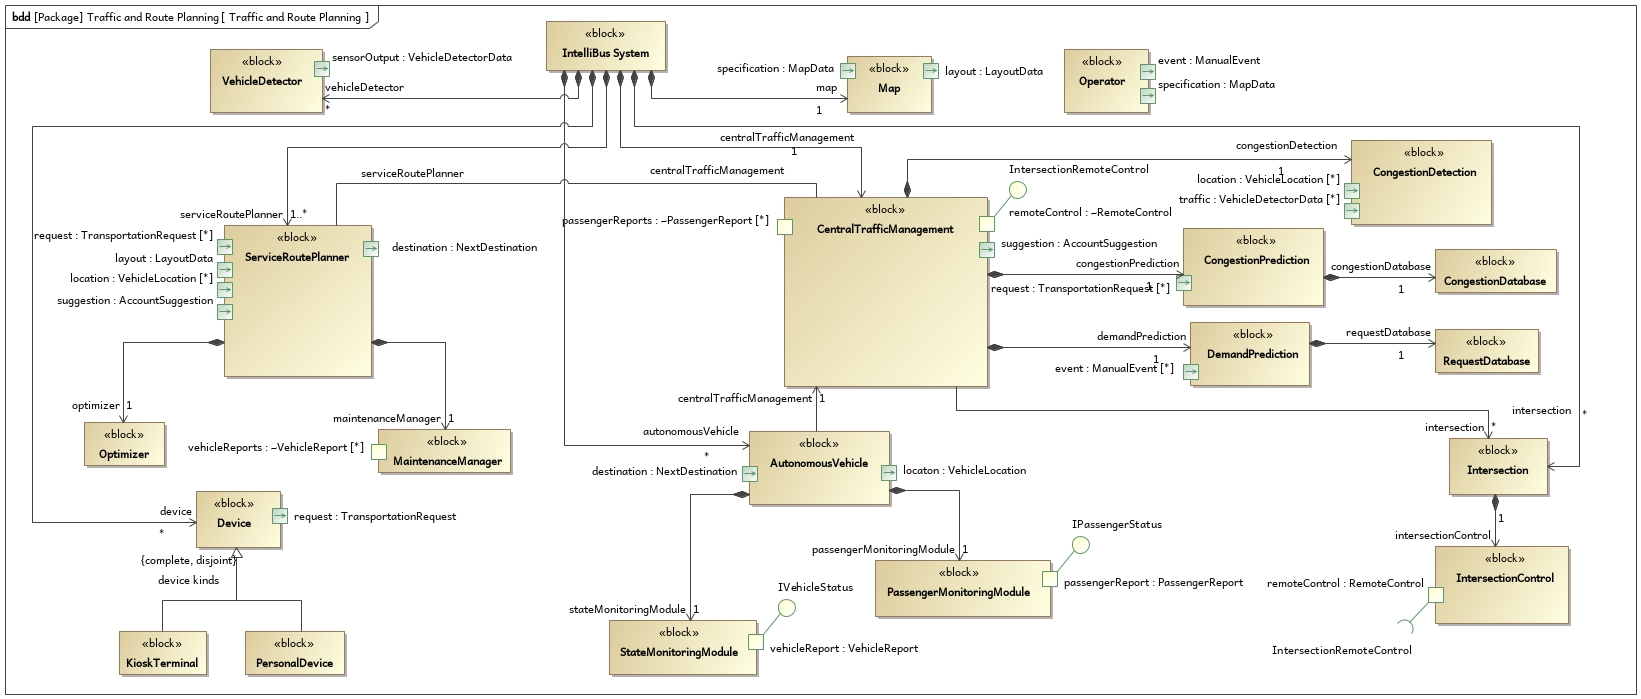
\includegraphics[width=\textwidth]{bdd-trp.jpg}
	\caption{Block Definition Diagram for the Traffic and Route Planning
		functionality}%
	\label{fig:bdd-trp}
\end{sidewaysfigure}

\begin{figure}
	\centering
	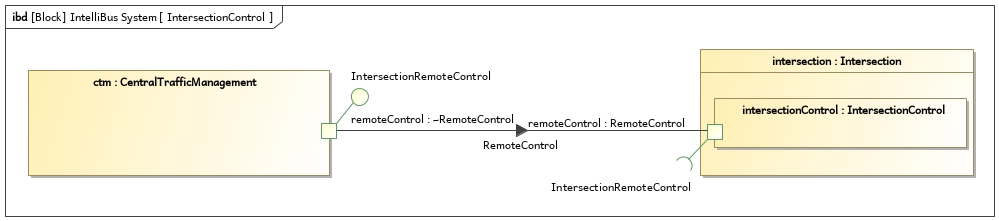
\includegraphics[width=\textwidth]{ibd-intersectioncontrol.jpg}
	\caption{Internal Block Diagram for the intersection control
		functionality}%
	\label{fig:ibd-intersectioncontrol}
\end{figure}

\begin{figure}
	\centering
	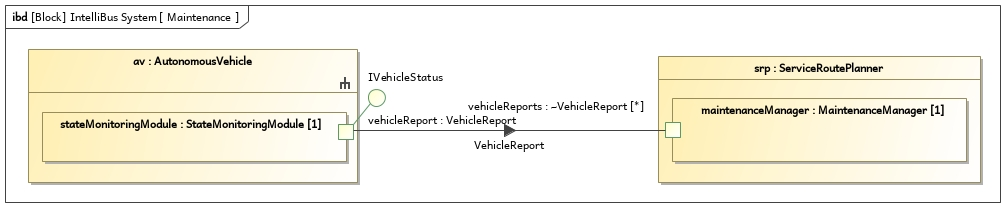
\includegraphics[width=\textwidth]{ibd-maintenance.jpg}
	\caption{Internal Block Diagram for the maintenance functionality}%
	\label{fig:ibd-maintenance}
\end{figure}

\begin{figure}
	\centering
	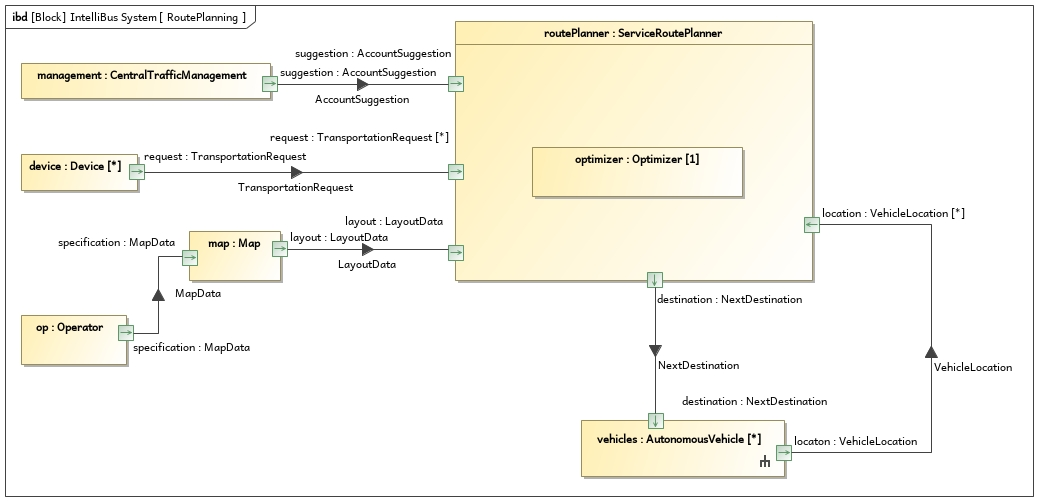
\includegraphics[width=\textwidth]{ibd-routeplanning.jpg}
	\caption{Internal Block Diagram for the route planning functionality}%
	\label{fig:ibd-routeplanning}
\end{figure}

\begin{sidewaysfigure}
	\centering
	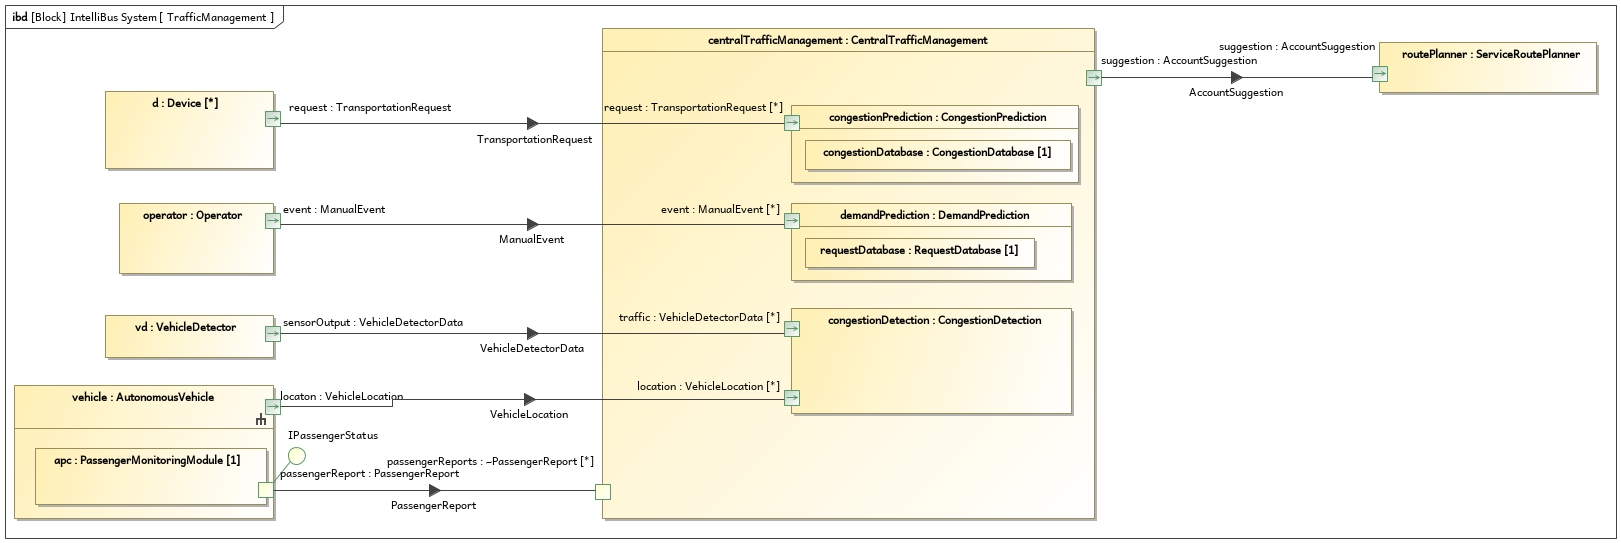
\includegraphics[width=\textwidth]{ibd-trafficmanagement.jpg}
	\caption{Internal Block Diagram for the traffic management
		functionality}%
	\label{fig:ibd-trafficmanagement}
\end{sidewaysfigure}

% - - - - - - - - - - - - - - - - - - - - - - - - - - - - - - - - - - - - - - -
%\subsection{Well-formedness constraints (iMSc)}

% TODO ?


% ------------------------------------------------------------------------------
\section{Work journal}

\begin{tabularx}{\textwidth}{l l l X}
	\toprule
	Team member & Date & Time\footnote{in hours} & Activity \\ \midrule

	everybody         & 2019-10-08 & 1.5 & meeting, planning              \\
	Borbála Szilágyi  & 2019-10-14 & 1   & extension of APC in MagicDraw  \\
	Borbála Szilágyi  & 2019-10-14 & 1   & TRP BDD sketch                 \\
	Annamária Gálik   & 2019-10-14 & 1   & glossary                       \\
	Bertalan Z. Péter & 2019-10-17 & 0.5 & IIC IBD sketch                 \\
	Bertalan Z. Péter & 2019-10-17 & 0.5 & IIC IBD in MagicDraw           \\
	Bertalan Z. Péter & 2019-10-17 & 0.5 & TRP BDD sketch                 \\
	Borbála Szilágyi  & 2019-10-18 & 2   & TRP BDD in MagicDraw           \\
	Bertalan Z. Péter & 2019-10-18 & 1   & IIC IBD fixes in MagicDraw     \\
	Borbála Szilágyi  & 2019-10-19 & 0.5 & TRP BDD fixes in MagicDraw     \\
	Annamária Gálik   & 2019-10-19 & 1.5 & TRP BDD fixes \& TRP IBD in
	                                       MagicDraw                      \\
	Bertalan Z. Péter & 2019-10-19 & 0.5 & IIC IBD fixes in MagicDraw     \\
	Borbála Szilágyi  & 2019-10-19 & 0.5 & documentation: our task and
	                                       ambiguities sections           \\
	Annamária Gálik   & 2019-10-19 & 1   & glossary extensions, also in
	                                       MagicDraw                      \\
	Borbála Szilágyi  & 2019-10-20 & 1   & TRP BDD finalization in
	                                       MagicDraw                      \\
	Borbála Szilágyi  & 2019-10-20 & 1.5 & TRP IBD fixes and finalization
	                                       in MagicDraw                   \\
	Bertalan Z. Péter & 2019-10-20 & 1.5 & documentation: the rest,
	                                       figures                        \\
	\bottomrule
\end{tabularx}

\clearpage
\glsaddall
\printglossaries

\end{document}
